% ====================
% 5. Evaluation and results
% ====================
\section{Evaluation and Results}
\label{sec:results}

\subsection{Evaluation Metrics}
\label{sec:metrics}

An LLM judge identifies the action taken in each
free-text answer. We report adherence (expected action selected),
pair accuracy (both A and B probes correct), the
retrieval--application gap (expected memory retrieved but wrong
action selected), retention (unrelated standing preference
followed), tag accuracy, and failure stage; Appendix~\ref{app:metrics}
gives the definitions.

Adherence is also separated into in-scope (A) and
out-of-scope (B) probes. Incorrect decisions are
classified as over-application, under-application,
supersession, or other actions.

Retrieval is checked by verbatim or judge-assisted
matching of rewritten notes; the full-transcript control
counts as retrieved by construction, and no memory as not
retrieved. Retention excludes unassessable answers.

Tagging accuracy is measured per field against the gold
labels on notes tied to one reference memory
(Appendix~\ref{app:metrics}).

Each incorrect answer is assigned to its earliest detected
failure stage (extraction, retrieval, scope loss, tagging, or
reasoning). These are diagnostic classifications, not
established causal mechanisms, and Supermemory's internal
extraction cannot be inspected separately from retrieval.

\subsection{LLM-as-a-Judge and Statistical Analysis}
\label{sec:judge}

The judge is the same Qwen model at temperature 0. It sees the
probe, response, and alphabetically ordered candidate actions
(not the expected action) and returns an action,
\texttt{none}, or \texttt{mixed}, with evidence; it also
evaluates the retention check.

The recorded human review covers 40 action labels
and 38 assessable retention labels, with complete
agreement against the judge (Cohen's
$\kappa=1.00$)~\cite{cohen1960coefficient}.
The judge and agent share a model, so correlated
errors remain possible; LLM-judge biases are
discussed by Zheng et al.~\cite{zheng2023judging}.

We report 95\% Wilson confidence intervals
\cite{wilson1927probable} and exploratory exact
McNemar tests~\cite{mcnemar1947sampling} on the
same episodes. Because the A/B probes within a
pair share history, episode-level tests do not
fully account for dependence; p-values are
interpreted cautiously. All 320 runs completed without
execution errors.

\subsection{Overall Correction Adherence}

Figure~\ref{fig:overall-adherence} shows adherence
across the eight conditions. No memory achieves
20\% (8/40), versus 80\% (32/40) with the full
transcript. Mem0 and Supermemory achieve 77.5\%
(31/40) and 85\% (34/40).

Read-time tagging achieves 80\% with Mem0 and
92.5\% (37/40) with Supermemory, the highest
observed score. Write-time tagging reduces
adherence to 60\% and 77.5\%, respectively.
Supermemory + read-time resolves 17/20 complete
pairs, compared with 15/20 for its baseline.
Its improvement is not statistically significant
under the reported McNemar test ($p=0.25$).

\begin{figure}[t]
\centering
\begin{minipage}[t]{0.45\linewidth}
\centering
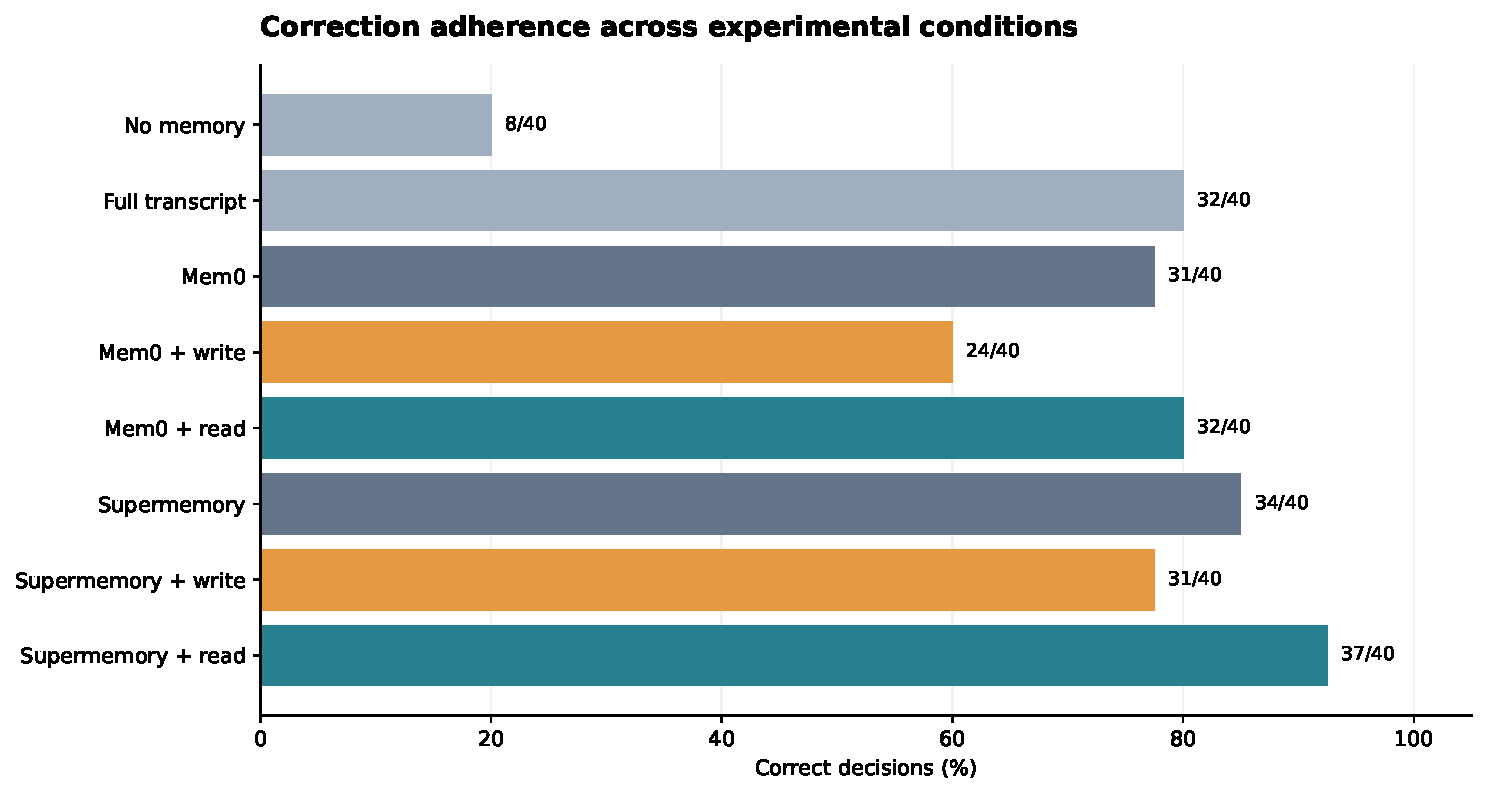
\includegraphics[width=\linewidth]{01_overall_adherence.pdf}
\caption{Correction adherence across eight conditions
(40 episodes per condition); error bars are 95\% Wilson
intervals.}
\label{fig:overall-adherence}
\end{minipage}\hfill
\begin{minipage}[t]{0.45\linewidth}
\centering
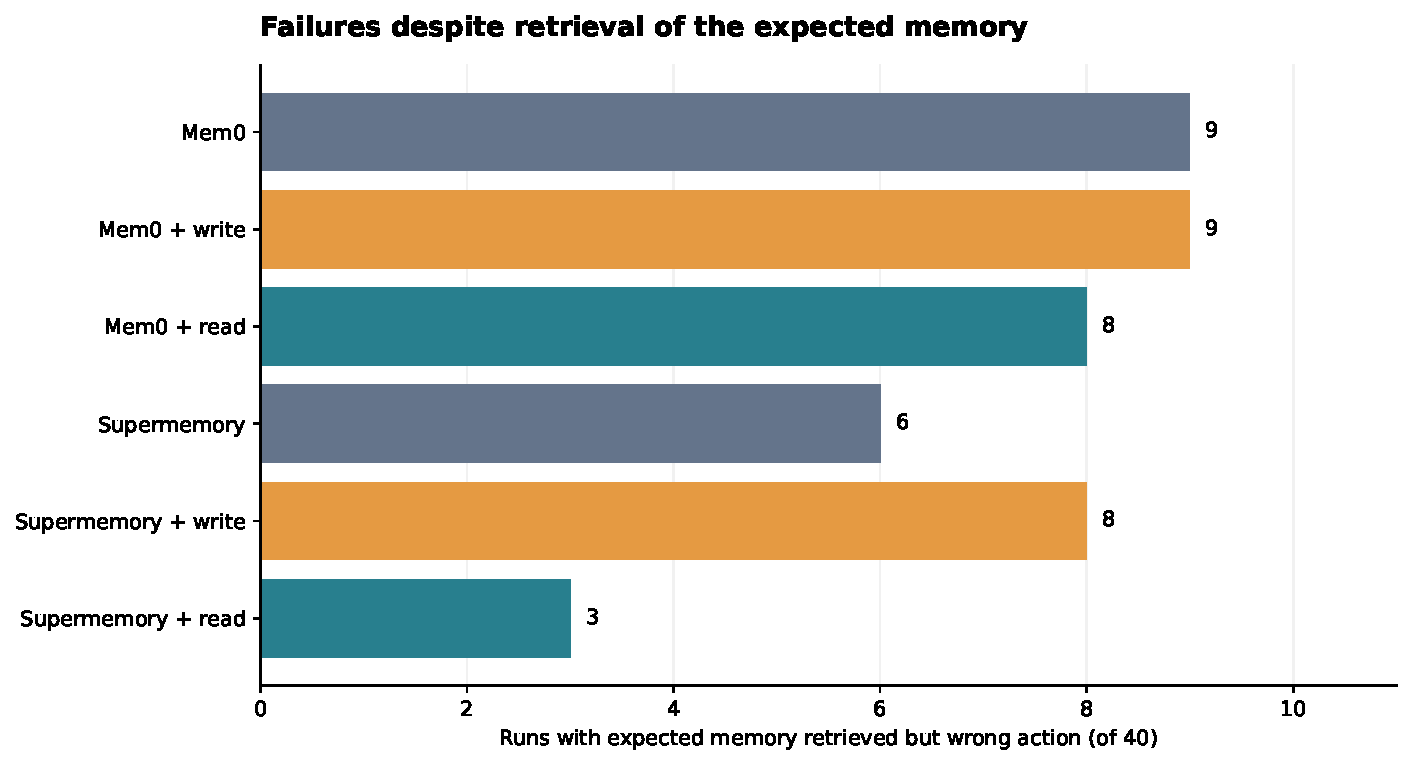
\includegraphics[width=\linewidth]{02_retrieved_but_wrong.pdf}
\caption{Incorrect actions despite retrieval
of the expected memory.}
\label{fig:retrieval-gap}
\end{minipage}
\end{figure}

\subsection{Retrieval Versus Application}

Across the six memory-system conditions, 43 of 51
incorrect responses occurred despite retrieval of
the expected memory (Figure~\ref{fig:retrieval-gap}).
Unmodified Mem0 and Supermemory retrieved the
expected memory in all 40 episodes but made nine
and six incorrect decisions, respectively.
Read-time tagging reduced these counts to eight
and three.

Successful retrieval is thus insufficient for correct
application, although a retrieved note may have lost scope
information.


\subsection{Scope-Boundary and Conflict-Type Performance}

Figure~\ref{fig:scope-boundaries} reveals asymmetric
write-time errors. Mem0 + write correctly handles
10/20 in-scope probes, versus 17/20 for Mem0.
Supermemory + write handles 11/20, versus 18/20
for its baseline, but correctly handles all 20
out-of-scope probes. This indicates substantial
under-application of scoped instructions.

Supermemory + read-time handles 20/20 in-scope
and 17/20 out-of-scope probes.

\begin{figure}[t]
\centering
\begin{minipage}[t]{0.45\linewidth}
\centering
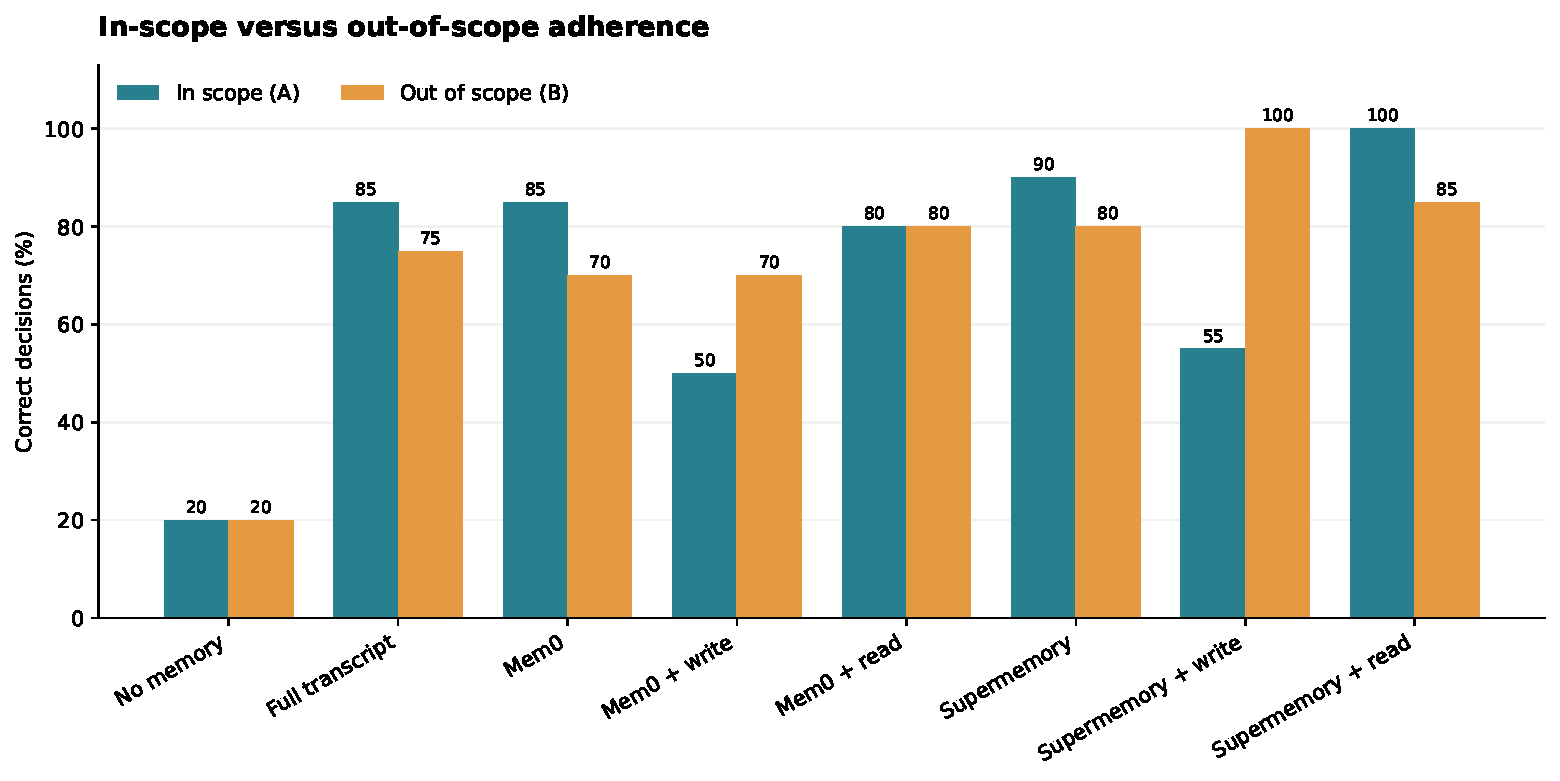
\includegraphics[width=\linewidth]{03_in_scope_vs_out_scope.pdf}
\caption{Adherence on in-scope (A) and out-of-scope
(B) probes, 20 of each per condition.}
\label{fig:scope-boundaries}
\end{minipage}\hfill
\begin{minipage}[t]{0.45\linewidth}
\centering
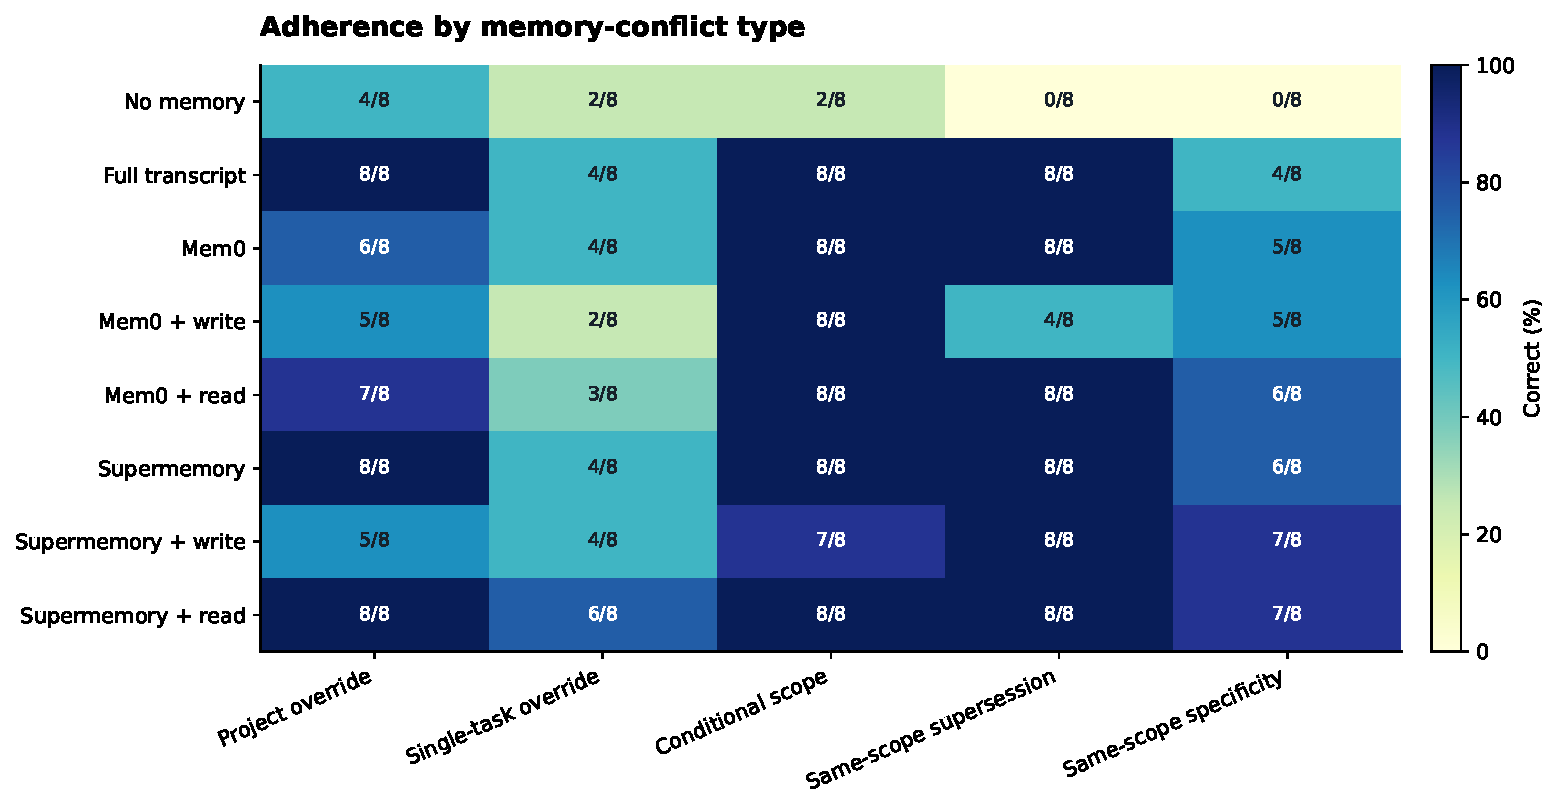
\includegraphics[width=\linewidth]{04_conflict_heatmap.pdf}
\caption{Adherence across five conflict categories;
eight episodes per category.}
\label{fig:conflict-types}
\end{minipage}
\end{figure}

Across conflict types (Figure~\ref{fig:conflict-types}),
conditional scope and same-scope supersession are
handled reliably by most memory-system conditions.
Single-task overrides are hardest: Mem0 and
Supermemory each achieve 4/8, while read-time
Supermemory reaches 6/8. Same-scope specificity
also remains challenging, with 4--7/8 correct
among the full-transcript and memory conditions.


\subsection{Failure Diagnosis, Tagging, and Retention}

The diagnostic breakdown in
Figure~\ref{fig:failure-stages} (Appendix~\ref{app:metrics}) attributes most
Supermemory baseline errors to reasoning despite
available information. Mem0 exhibits five baseline
scope-loss errors; write-time Mem0 has seven
extraction and four tagging failures among its
16 incorrect responses. Supermemory + write-time
has eight reasoning-classified failures among nine.

Write-time tagging achieves 100\% scope accuracy
on evaluated tags for both systems, versus 87\%
for read-time Mem0 and 77\% for read-time
Supermemory. Nevertheless, the highest downstream
adherence occurs with read-time Supermemory,
illustrating that tag accuracy alone is insufficient.
These figures use different eligible-note sets
and are not directly controlled comparisons.

Unrelated-memory retention is 95\% with the full
transcript, 67.5\% with Mem0 (significantly lower,
$p=0.003$), and 97.5\% with Supermemory. Scope-aware
Mem0 variants retain 62--72\%, compared with 87--98\%
for Supermemory variants; tagging does not change
retention significantly for either system.

